\documentclass{beamer}
\usepackage{listings}
\lstset{
%language=C,
frame=single, 
breaklines=true,
columns=fullflexible
}
\usepackage{subcaption}
\usepackage{url}

\usepackage{tikz}
\usepackage{pgfplots}
\pgfplotsset{compat=1.17}
\usepackage{tkz-fct}
\usepackage{mathrsfs}
\usepackage{txfonts}
\usepackage{tkz-euclide} 
\usetikzlibrary{calc,math}
\usepackage{float}
\newcommand\norm[1]{\left\lVert#1\right\rVert}
\renewcommand{\vec}[1]{\mathbf{#1}}
\providecommand{\pr}[1]{\ensuremath{\Pr\left(#1\right)}}
\usepackage[export]{adjustbox}
\usepackage[utf8]{inputenc}
\usepackage{amsmath}
\usetheme{Boadilla}
\title{Research Paper Presentation}
\author{Tanmay Garg - EE20BTECH11048}

\begin{document}
\begin{frame}
\titlepage
\end{frame}
\section{}
\begin{frame}{Performance analysis of M-QAM OFDM for satellite laser communication systems}
\begin{block}{Abstract}
\begin{enumerate}
    \item We will talk about a satellite laser communication system based on M-QAM and OFDM and analyze its performance.
    \item The relationship between the link bit error rate and the transmission power under different conditions of atmospheric turbulence and M-QAM modulation.
    \item The results have shown that as the turbulence intensity increases, the QAM modulation of order M increases, and the performance of OFDM optical links continues to deteriorate.
\end{enumerate}

\end{block}
\end{frame}
\section{Introduction}
\begin{frame}{Keywords and some definitions}
\begin{block}{Modulation}
   It is the process where the properties of a carrier wave such as amplitude, frequency and phase is changed according to the information signal.
\end{block}
    \begin{block}{Orthogonal Frequency Division Multiplexing Modulation (OFDM):}
   Method of encoding digital data on multiple carrier frequencies, instead of a single wide frequency bandwidth.
    \end{block}
    \begin{block}{Frequency Selective Fading}
     Anomaly caused by partial cancellation of a radio signal by itself
    \end{block}
    \begin{block}{Quadrature Amplitude Modulation (QAM):}
       It utilises both amplitude and phase components that is able to provide high levels of spectrum usage efficiency
    \end{block}
\end{frame}
%\begin{frame}{Keywords}
%\begin{block}{Quadrature Amplitude Modulation (QAM):}
%       It utilises both amplitude and phase components that is able to provide high levels of spectrum usage efficiency
%    \end{block}
%    \begin{block}{Phase Shift Keying (PSK):}
%       A digital modulation process which conveys data by modulating the phase of a constant frequency carrier wave.
%    \end{block}
%\end{frame}
\section{Structure Principle}
\begin{frame}{Structure Principle}
\begin{block}{Block Diagram}
\begin{figure}
    \centering
    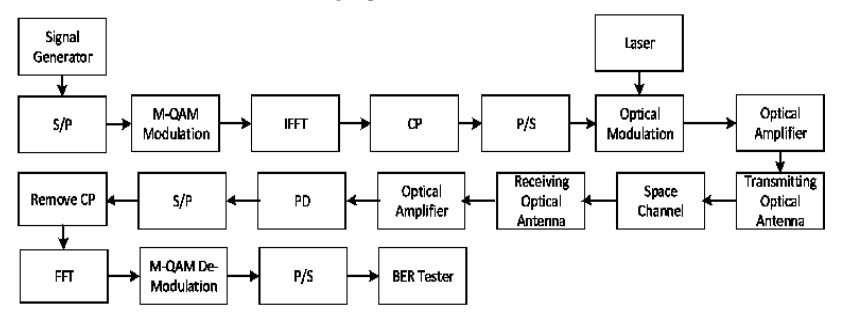
\includegraphics[width=\columnwidth]{block_diagram.png}
    \caption{MQAM OFDM Structure Principle}
    \label{fig:my_label}
\end{figure}
\end{block}
\end{frame}
\begin{frame}{Structure Principle}
\begin{block}{Block Diagram Components}
\begin{enumerate}

    \item S/P: Serial to Parallel Converter converts datastream from series to N parallel parts which form each subcarrier for easy modulation and using the frequency spectrum optimally
    \item MQAM modulation means $M$ symbols are used to represent and transmit data and each symbol is given a certain percentage of amplitude and phase difference
    \item IFFT is inverse fast Fourier transform which modulates the info signal onto carrier signal to give modulated signal
    \item Space Channel is the medium through which the signal will be transmitted.
    %\item a single channel utilizes multiple sub-carriers on adjacent frequencies. In addition the sub-carriers in an OFDM system are overlapping to maximize spectral efficiency. sub-carriers in an OFDM system are precisely orthogonal to one another.
    
\end{enumerate}
\end{block}

\end{frame}

\begin{frame}{Structure Principle}
\begin{block}{Block Diagram components}
\begin{enumerate}
    \item Optical Modulation allows one to control an optical wave or to encode information on a carrier optical wave.
    \item A cyclic prefix is a repetition of the first section of a symbol that is appended to the end of the symbol
        \item A Photo Detector detects the required electromagnetic radiation  and converts them to electrical signals.
        \item BER tester is the Bit Error Rate tester.
    \end{enumerate}
\end{block}
    
\end{frame}
\section{Space Channel}
\begin{frame}{Space Channel}
\begin{block}{About Space Channel}
\begin{enumerate}
    \item It is the medium through which the entire signal is transmitted.
    \item There is a lot of interference from other signals, atmospheric turbulence, noise and attenuation.
    \item Many different statistical models have been proposed for light intensity flicker caused by atmospheric turbulence. Eg\begin{enumerate}
        \item Negative exponential distribution
        \item Lognormal distribution
        \item Gamma-Gamma distribution model
    \end{enumerate}
\end{enumerate}
\end{block}
\end{frame}


\begin{frame}{Gamma Gamma Distribution Model}
    \begin{block}{PDF}
    \begin{align}
    f_{h_t}(h_t)&=\frac{2(\alpha \beta)^{\frac{\alpha+\beta}{2}}}{\Gamma{(\alpha)} \Gamma{(\beta)}}{(h_t)}^{(\frac{\alpha+\beta}{2}-1)}K_{\alpha-\beta}\sqrt{2\alpha\beta h_t}\\
    \alpha &= \left\{\exp{\left[\frac{0.49\sigma_0^2}{\left(1 +1.1\sigma_0^{\frac{12}{5}}\right)^\frac{7}{6}}\right]}-1\right\}^{-1} \label{alpha_eq}\\
    \beta &= \left\{\exp{\left[\frac{0.51\sigma_0^2}{\left(1 +0.69\sigma_0^{\frac{12}{5}}\right)^\frac{5}{6}}\right]}-1\right\}^{-1} \label{beta_eq}
\end{align}
    \end{block}
\end{frame}
\begin{frame}{Gamma Gamma Distribution Model}
    \begin{block}{PDF}
    \begin{table}[]
        \centering
\renewcommand{\arraystretch}{1.4}
        \begin{tabular}{|c|c|}
        \hline
             Parameter& Parameter Denotes \\ \hline
            $K_{\alpha-\beta}\sqrt{2\alpha\beta h_t}$ & Second class modified Bell Function:order  $\alpha-\beta$\\ \hline
            $\sigma_0^2=1.23C^2K^\frac{7}{6}z^\frac{11}{6}$&Rytov Variance\\ \hline
             $C_n^2$&Atmospheric refractive index structural constant\\ \hline
             $K=\frac{2\pi}{\lambda}$&plane wave number\\ \hline
             $z$ & speed of light\\ \hline
             $\Gamma(\alpha) \Gamma(\beta)$ & Gamma function\\
             \hline
        \end{tabular}
        \caption{Parameters}
        \label{tab:my_label}
    \end{table}
    \end{block}
\end{frame}
\begin{frame}{Gamma Gamma Distribution Model}
\begin{block}{Important Points}
\begin{enumerate}
\item $h_t$ is our random variable for which distribution is plotted.
    \item $\alpha$ and $\beta$ are defined according to \eqref{alpha_eq} and \eqref{beta_eq} and depend on $\sigma_0$ 
    \item$\sigma_0$ depends on the medium through which the wave passes and wave-number of link operating wave.
    \item $\sigma_0$ also depends on the speed of light which may vary depending upon the atmospheric condition and the medium.
    
\end{enumerate}
\end{block}
\end{frame}
\begin{frame}{Pointing Error}
    \begin{block}{Pointing error theory}
    Along with atmospheric turbulence, the pointing errors of the optical links between the platforms affect the fluctuation of the optical signal intensity.
    \end{block}
    \begin{block}{PDF}
    Probability density function of the pointing error factor of the optical link between platforms:
    \begin{align}
        f_{h_p}(h_p)&=\frac{\xi^2}{A_0^{\xi^2}}(h_p)^{(\xi^2-1)}, \quad {0\leq h_p \leq A_0}\\
        \nu&=\frac{\sqrt{\pi r}}{\sqrt{2}w_z}\\
    \xi &= \frac{w_{z,eq}}{2\sigma_s}
    \end{align}
    \end{block}
\end{frame}
\begin{frame}{Pointing error}
\begin{block}{PDF}
\begin{table}[]
    \centering
    \renewcommand{\arraystretch}{1.3}
    \begin{tabular}{|c|p{0.68\columnwidth}|}
    \hline
    Parameter & Parameter Denotes\\ \hline
         $w_{z,eq}^2=\frac{w_z^2\sqrt{\pi}erf(\nu)}{2\nu\exp{(-\nu^2)}}$& Equivalent beam width at the receiving end\\ \hline
         $\sigma_s$& Standard deviation of pointing error offset at receiving end\\ \hline
         $erf(\nu)$& Error Function\\ \hline
         $w_z =\theta z$& Beam width at distance $z$\\ \hline
         $z$ & distance between transmitter and receiver\\ \hline
         $\theta$& Beam emission angle\\ \hline
        $r$ &Receiver Radius\\
         \hline
    \end{tabular}
    \caption{Parameters}
    \label{tab:my_label_2}
\end{table}
    
\end{block}
    
\end{frame}
\subsection{Demodulation}
\begin{frame}{Demodulator}
    \begin{block}{Performing demodulation}
    \begin{enumerate}
        \item The data is converted to parallel and cyclic prefix is removed. FFT is applied.
        \item $N$ symbol data is now $N+L$ symbol data, due to IFFT and adding CP.
        %\item The OFDM signal is produced by taking the IFFT of modulated signal at baseband. 
        \item Suppose the required period of an OFDM symbol is T. 
        \item At the beginning of every OFDM symbol there is a cyclic prefix of length $T_g$ , created by taking last $L$ symbol in a OFDM sysmbol and adding to begining. 
        \item $T_g$ must be greater than channel impulse response time to be useful. 
    \end{enumerate}
    \end{block}
\end{frame}
\begin{frame}{Subcarrier}
\begin{block}{Formula}
\begin{align}
    \nu(t)=\sum_{k=-N}^N C_k \exp{(2\pi jf_kt)}, \quad {0 \leq t\leq T}
\end{align}
\begin{enumerate}
    \item $f_k=\frac{k}{T}$ the frequencies of complex exponential
    \item At the receiver it is down converted, timing synchronization is done, cyclic prefix is removed and FFT is applied.
\end{enumerate}
\end{block}
    
\end{frame}
\begin{frame}{How error occurs?}
\begin{figure}
    \centering
    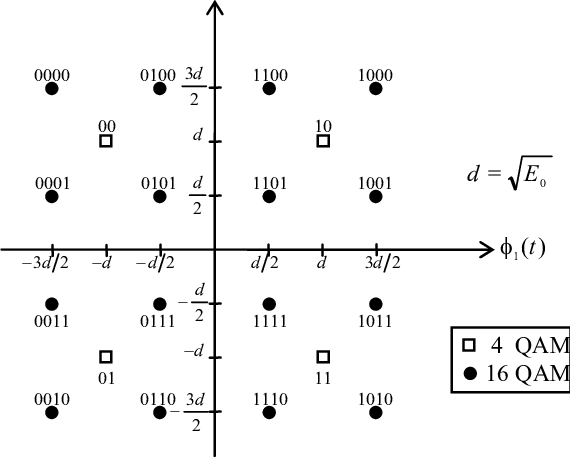
\includegraphics[width=0.6\columnwidth]{Constellation-diagram-for-square-MQAM-with-Gray-encoding-illustrated-for-M-4-and-M.png}
    \caption{Mapping symbols in phase and amplitude}
    \label{fig:constlation}
\end{figure}
    
\end{frame}
\section{Experiment}
\begin{frame}{Experiment and Results}
    \begin{block}{Case 1}
Sub-carrier uses 4-QAM modulation. Turbulence strengths $\sigma_0^2$ is taken as 0.4,1.4 and 4.
\begin{figure}
    \centering
    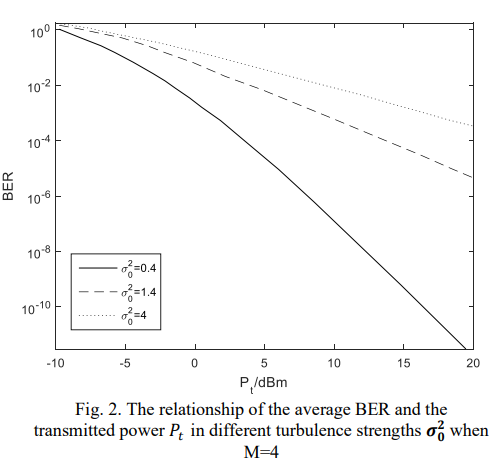
\includegraphics[width = 0.4\columnwidth]{fig2.png}
    \caption{}
    \label{fig:fig2_lab}
\end{figure}
    \end{block}
\end{frame}

\begin{frame}{Experiment and Results}
    \begin{block}{Case 2}
Turbulence strength $\sigma_0^2 = 1.4$ and different M-QAM modulations are taken for 4,16, and 64. 
\begin{figure}
    \centering
    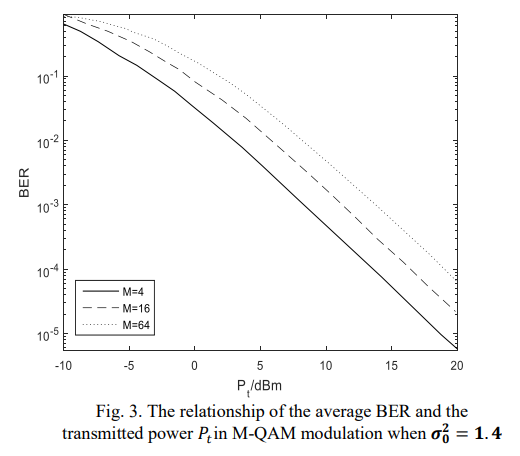
\includegraphics[width = 0.4\columnwidth]{fig3.png}
    \caption{}
    \label{fig:fig2_lab}
\end{figure}
    \end{block}
\end{frame}
\begin{frame}{Experiment and Results}
\begin{block}{Results}
\begin{enumerate}
\item The relationship between the bit error rate of an OFDM link and the transmit power under different atmospheric turbulence conditions and for different M-QAM modulation.
    \item In first case, as the turbulence intensity increases the BER also increases and the performance decreases. By increasing the transmitting power, BER decreases.
    \item In second case, as the order M increases the BER also increases and the performance decreases. By increasing the transmitting power, BER decreases.
\end{enumerate}
\end{block}
    
\end{frame}
\section{Conclusion}
\begin{frame}{Conclusion}
    \begin{block}{Conclusions and Inference}
    \begin{enumerate}
        \item MQAM OFDM is applied to satellite laser 
communication.
\item The relationship between the bit error rate 
of the OFDM optical link and the transmission power is 
analyzed under different conditions.
\item The results show that as the turbulence intensity increases, the 
QAM modulation order M increases, and the performance of 
OFDM optical links continues to deteriorate.
\item This gives us the reference for optimization of OFDM in satellite laser communication.
    \end{enumerate}
    \end{block}
\end{frame}
\end{document}